\chapter{Introdução}
O setor energ\'{e}tico \'{e} de suma import\^{a}ncia para qualquer pa\'{i}s. Com o decorrer das \'{u}ltimas d\'{e}cadas a sociedade de 
um modo geral ser tornou altamente  dependente da energia el\'{e}trica. A preocupa\c{c}\~{a}o em supir essa demanda crescente por energia levou
ao surgimento de modelos para o planejamento de dispacho de energia, tais modelos devem ser ajustar adequadamente ao planejamento energ\'{e}tico.
Portanto, n\~{a}o \'{e} coincid\^{e}ncia que na constru\c{c}\~{a}o de ta\'{i}s modelos sejam o necess\'{a}rio o conhecimento de v\'{a}rias
\'{a}reas da ci\^{e}ncia. Dentre as quais tem-se a Matem\'{a}tica, Engenharia, Probabilidade e Hidrologia. Contudo, h\'{a} tamb\'{e}m uma 
preocupa\c{c}\~{a}o ambiental,pois, as a\c{c}\~{o}es do ser humano em sua maioria trazem  um impacto negativo sobre o ambiente, como \'{e} o caso
da gera\c{c}\~{a}o de energia termoel\'{e}trica e nuclear. Diante disso, metodologias que permitem o uso da energia el\'{e}trica de modo
eficiente, e a sua gera\c{c}\~{a}o constituem problemas de grande interesse. O Brasil pelo seu vasto territ\'{o}rio de natureza
continental e pela sua natureza clim\'{a}tica diferenciada tem uma posi\c{c}\~{a}o privilegiada para fontes de energias renov\'{a}veis.
\abbrev{ANELL}{Ag\^{e}ncia Nacional de Energia El\'{e}trica} Segundo a Ag\^{e}ncia Nacional de Energia El\'{e}trica (ANELL) no Brasil a principal
fonte de gera\c{c}\~{a}o de energia \'{e} hidroel\'{e}trica que corresponde a $62\%$, o restante \'{e} $28\%$ proveniente da gera\c{c}\~{a}o
t\'{e}rmica (g\'{a}s natural, carv\~{a}o mineral, comb\'{u}stiveis f\'{o}sseis, biomassa e nuclear) e  $10\%$ proveniente de gera\c{c}\~{a}o
e\'{o}lica e importa\c{c}\~{a}o de outro pa\'{i}ses. O processo b\'{a}sico para o dispacho de energia \'{e} constituido por tr\^{e}s etapas.
As respons\'{a}veis pela gera\c{c}\~{a}o de energia as \textit{geradoras}, as respons\'{a}veis pela transmiss\~{a}o de energia para os centros
urbanos as \textit{transmissoras} e por \'{u}ltimo as respons\'{a}veis por distribuir a energia para o consumidor final as \textit{distribuidoras}. 
\begin{figure}[!tb]
\centering
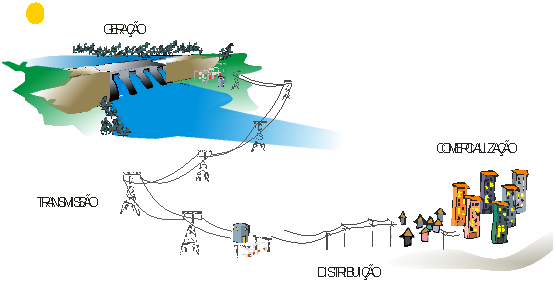
\includegraphics[scale=1.0]{./imagens/ANELL.png}
\caption{Dispacho de energia ANELL}
\label{energia}
\end{figure}
\newpage
\noindent
Percebe-se que qualquer problema envolvendo as geradoras t\^{e}m repercuss\~{o}es para os outros est\'{a}gios, ocasionado-se um aumento do
pre\c{c}o da tarifa de energia para o usu\'{a}rio final, portanto para um planejamento eficaz as geradoras tem um papel fundamental levando-se
em rela\c{c}\~{a}o fatores como o custo da produ\c{c}\~{a}o de energia el\'{e}trica. Por outro, lado o fator ambiental jamais deve ser esquecido.
Diante dessas condi\c{c}\~{o}es a serem consideradas, o Brasil, pela sua diversidade de recursos para a gera\c{c}\~{a}o de energia, tem-se 
utilizado a gera\c{c}\~{a}o mista,onde o modelo que ser destacar e o modelo hidrot\'{e}rmico. O modelo hidrot\'{e}rmico \'{e} constitu\'{i}do por 
usnas hidroel\'{e}tricas em cascata, onde caso tendo-se um n\'{i}vel de reservat\'{o}rio baixo para a demanda do sistema as t\'{e}rmicas associadas
s\~{a}o ativadas para supir a demanda de energia. As princiais dificuldades relacionadas a este tipo de modelo podem ser relaciondas pelo
uso de t\'{e}rmica cujo o custo tanto para a gera\c{c}\~{a}o, quanto para o meio ambiente e relativamente alto. Contudo, a gera\c{c}\~{a}o
t\'{e}rmica possui a vantagem de ter uma deped\^{e}ncia menor a fatores externos, comparada  h\'{a} outras fontes de energia, fazendo que sua
utiliza\c{c}\~{a}o seja necess\'{a}ria. A grande vantagem da gera\c{c}\~{a}o el\'{e}trica est\'{a} em seu custo relativamente baixo em
rela\c{c}\~{a}o as outras fontes de energia, por\'{e}m est\'{a} \'{e} altamente depedente do n\'{i}vel do reservat\'{o}rio. Tendo em vista tais
quest\~{o}es uma metodologia desenvolvida para trabalhar com tais dificuldades do modelo hidrot\'{e}rmico para a tomada de decis\~{a}o \'{e}
a modelagem hidrot\'{e}rmica baseada na \abbrev{PPDE}{Programa\c{c}\~{a}o Din\^{a}mica Est\'{o}catica}Programa\c{c}\~{a}o Din\^{a}mica
Dual Est\'{o}castica (PDDE), sendo, a base para  modelos como o DECOMP utilizado pela ANELL.



